\documentclass[backaddress=true,fromlogo=true]{scrlttr2}
\usepackage[utf8x]{inputenc}
\usepackage{color,calc,ngerman,mathptmx}
\usepackage{eurosym}
\usepackage{booktabs}
\usepackage{graphicx}

\renewcommand{\familydefault}{\sfdefault}

\setkomavar{fromname}{fnordeingang e.V.\\c/o Jan Krings}
\setkomavar{fromaddress}{Eichendorffstr. 44\\41464 Neuss}
\setkomavar{subject}{Beitragsrechnung}
\setkomavar{place}{Neuss}
\setkomavar{fromlogo}{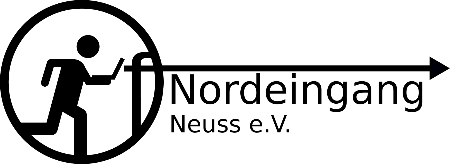
\includegraphics[scale=0.5]{logo}}


\firsthead{
\raisebox{-\totalheight}{%
      \usekomavar{fromlogo}}%
\null\hfill
  \parbox[t][\headheight][t]{6cm}{%
   \raggedright
   \color[gray]{.5}%
   \usekomavar{fromname}\\
   \usekomavar{fromaddress}\\[\baselineskip]
 %  \usekomavar*{fromphone}\\[\baselineskip]
   E-Mail:\hfill verein@fnordeingang.de\\
   Webseite:\hfill https://fnordeingang.de\\[\baselineskip]
   }%
}


\setkomavar{location}{
\\[\baselineskip]
\\[\baselineskip]
  \large{Rechnung Nr.\hfill 199}\\
  \large{Mitglied Nr.\hfill 10006}\\
  \large{Datum\hfill 28.04.2013}\\
}
\begin{document}
\setlength{\parindent}{0pt}
% If you want headings on subsequent pages,
% remove the ``%'' on the next line:
% \pagestyle{headings}

\begin{letter}{Max Mustermann\\Musterstr. 12\\41460 Neuss}
\opening{}
\renewcommand{\arraystretch}{1.3}

\baselineskip=12pt
\begin{tabular*}{\textwidth}{ccp{0.54\textwidth}rr}
  \textbf{Pos} & \textbf{Menge} & \textbf{Bezeichnung} & \textbf{Einzelpreis} & \textbf{Betrag} \\
 \hline
 1 & 1 Mnt & Mitgliedsbeitrag - Normal & \EUR{10,00} & \EUR{10,00}\\
 \hline
 \multicolumn{4}{r}{\rule{0pt}{4ex}Nettobetrag} & \multicolumn{1}{r}{\EUR{10,00}}\\[-4pt]
 \multicolumn{4}{r}{Umsatzsteuer 0\% (Steuerfreie Produkte)} & \multicolumn{1}{r}{\EUR{0,00}}\\
 \hline
 \multicolumn{4}{r}{\rule{0pt}{4ex}Endbetrag} & {\EUR{10,00}}\\
\end{tabular*}
\\
%Im ausgewiesenen Betrag ist gemäß §19 UStG keine Umsatzsteuer enthalten. \\
[\baselineskip]
\\
Zahlbar bis 29.04.2014 ohne Abzug.
\\
\\
Bankverbindung: Konto 93421964 • BLZ 30550000 • Sparkasse Neuss
\end{letter}
\end{document}
